%
% File acl2014.tex
%
% Contact: koller@ling.uni-potsdam.de, yusuke@nii.ac.jp
%%
%% Based on the style files for ACL-2013, which were, in turn,
%% Based on the style files for ACL-2012, which were, in turn,
%% based on the style files for ACL-2011, which were, in turn, 
%% based on the style files for ACL-2010, which were, in turn, 
%% based on the style files for ACL-IJCNLP-2009, which were, in turn,
%% based on the style files for EACL-2009 and IJCNLP-2008...

%% Based on the style files for EACL 2006 by 
%%e.agirre@ehu.es or Sergi.Balari@uab.es
%% and that of ACL 08 by Joakim Nivre and Noah Smith

\documentclass[11pt]{article}
\usepackage{acl2014}
\usepackage{times}
\usepackage{url}
\usepackage{latexsym}
\usepackage{graphicx}


%\setlength\titlebox{5cm}

% You can expand the titlebox if you need extra space
% to show all the authors. Please do not make the titlebox
% smaller than 5cm (the original size); we will check this
% in the camera-ready version and ask you to change it back.


\title{LING 573 Multi-Document Summarization}

\author{Emma Bateman \\
  {\tt email@domain} \\\And
  John Dodson \\
  {\tt jrdodson@uw.edu} \\\And
  Charlie Guo \\
  {\tt email@domain}
  }

\date{}

\begin{document}
\maketitle
\begin{abstract}
We describe an unsupervised multi-document summarization system using TextRank, a graph-based algorithm for ranking salient sentences in a corpus of text documents. The system is divided into three primary components for selecting content, generating feature representations, and ranking significant features for summary generation.
\end{abstract}

\section{Introduction}

Multi-document summarization systems seek to aggregate collections of text documents and condense their content to provide cohesive summaries. Traditional approaches to summarization fall into two distinct categories: abstractive and extractive. Abstractive techniques are categorized based on their ability to generate novel summary content, in contrast with extractive approaches which select significant content directly from the source documents. In this work, we present an unsupervised system for extractive multi-document summarization over a benchmark dataset. The system is centered around the TextRank algorithm, which is a graph-based technique to identify and rank the most salient sentences in the input documents. We evaluate our system on the AQUAINT and AQUAINT-2 corpora, with average ROUGE-1 and ROUGE-2 F-scores of $0.26093$ and $0.06952$, respectively. 

This report is structured as follows: Section 2 provides an overview of our system and its components, including a description of the AQUAINT dataset; section 3 details our approach to generating summaries using TextRank and creating feature vectors from the raw sentences; section 4 presents result metrics; section 5 is a discussion of the approach and details potential improvements to the baseline system; section 6 concludes.

\section{System Overview}
The system is divided into three primary components: a content selector, a feature extractor, and a ranker. The content selector is responsible for ingesting a schema file which details one or more document clusters in the AQUAINT datasets. The selector identifies which documents belong together in a cluster and then ingests those documents as plain text. The feature extractor tokenizes the text at the sentence level and generates feature vectors per sentence. The feature vectors are given as input to the ranking algorithm which runs TextRank to sort vectors by significance. 

\subsection{Architecture}
\begin{figure}
  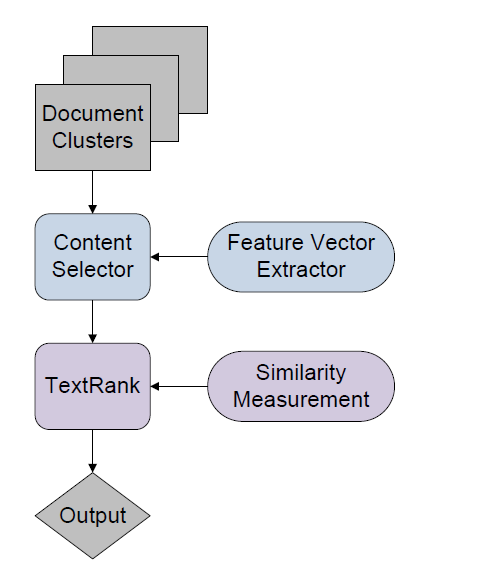
\includegraphics[width=\linewidth]{arch.PNG}
  \caption{Multi-document summarization system architecture}
  \label{fig:arch}
\end{figure}

Figure \ref{fig:arch} provides an illustration of the existing system architecture. No training is required to generate summaries from text documents, only properly formatted schema files which provide document cluster information.

\section{Approach}

This section provides detail into the three main components of the working system.

\subsection{Content Selection}
The ingest processor for the system consumes one or more documents associated with a cluster identifier. These SGML documents are converted to plain text and represented as a single monolithic text string. After ingest is complete, the system will maintain one text representation per document cluster.

The system uses BeautifulSoup to perform most of its SGML and XML parsing. For a given input file, the ingest processor identifies clusters and their associated documents by finding document IDs which correspond to AQUAINT SGML files. The system then loads the corresponding SGML files and pefrorms traversal using BeautifulSoup to find the appropriate blocks of text.
\subsubsection{Feature Vectors}
The feature extraction component takes the plain text representation and tokenizes it into individual sentences using Python's Natural Language Toolkit (NLTK). NLTK is used to remove common stopwords from each sentence. Feature vectors are generated in two steps: firstly, the component identifies a comprehensive vocabulary for the cluster; and secondly, a frequency vector is created based on the token frequencies in the given sentence. 

The output of this component is an $N$ x $V$ matrix, where $N$ is the total number of sentences in the cluster and $V$ is the size of the vocabulary. 
\subsubsection{TextRank}
Our system uses TextRank to compute saliency scores for each sentence in the cluster and subsequently rank them according to significance. The TextRank algorithm constructs a graphical representation of textual features, where a given textual feature is represented as a vertex in the graph. The algorithm assigns a significance score to each vertex based on inbound edge weighting.

The authors of the TextRank algorithm formally define a graph as a tuple $G = (V,E)$, where $V = \{v_1, v_2, ... v_n\}$ is the set of vertices in the graph and $E$ is a set of edges and a subset of $V$ x $V$. TextRank is inspired by PageRank and computes the score for some vertex $V_i$ similarly to the original algorithm:
\begin{center}
    $S(V_i) = (1 - d) + d * \sum_{j \in In(V_i)} \frac{1}{|Out(V_j)|}S(V_j)$
\end{center}
$In(V_i)$ represents all inbound connections to vertex $V_i$, and $Out(V_j)$ represents outbound connections from vertex $V_j$. The authors use $d$ as a damping factor set between $0$ and $1$, which effectively biases the calculation. The original PageRank algorithm defaults this factor to $0.85$, and in our system we maintain this defaulted value.

In applying TextRank to sentence processing, we compute a pairwise similarity matrix of size $N$ x $N$, where $N$ is the total number of sentences in the cluster. The similarity between $N_i$ and $N_j$ becomes the edge weight which connects those two vertices in the graph. We use cosine similarity as our distance measurement.

After the TextRank algorithm converges, the algorithm returns the top K sentences as the cluster summary. Each summary contains 100 words maximum. The system maintains a reference to the original sentences, and uses the original text as output. We cleanse the summaries by stripping trailing newlines, and order the outputs as one sentence per line.
\section{Results}

Results TBD

\section{Discussion}

Discussion TBD


\section{Conclusion}
 We have described an unsupervised system for generating single summaries over multiple documents. The system generates feature vectors per sentence by computing word frequencies, and then provides those frequency vectors as input to the TextRank algorithm. The algorithm is able to identify significant lines of text in a single pass. We take the top K sentences as the corresponding summary, up to 100 words max per summary.

% include your own bib file like this:
%\bibliographystyle{acl}
%\bibliography{acl2014}

\begin{thebibliography}{}

\bibitem{textrank04}
	Rada Mihalcea and Paul Tarau,
	\textit{TextRank: Bringing Order into Texts},
	Proceedings of the 2004 Conference on Empirical Methods in Natural Language Processing,
	2004.

\end{thebibliography}

\end{document}